% !TEX root =main.tex

\section{Evaluation}\label{sec::eval}


%In this section, we analyse the asymptotic costs and run-time of  the PwDR protocol. 







\subsection{Asymptotic Cost Analysis} In this section, we evaluate the PwDR protocol’s computation and communication complexity. Table \ref{table::PwDR-Asymptotic-Cost} summarises the result. 

% !TEX root =main.tex


 \begin{table*}[!htb]

\caption{ \small The PwDR protocol's asymptotic cost. In the table, $n$ is the  number of arbiters and $e$ is the threshold.} \label{table::PwDR-Asymptotic-Cost} 
 \vspace{-2mm}
\begin{center}

\begin{tabular}{|c|c|c|c|c|} 

   \hline
   


\multirow{2}{*}{\scriptsize \textbf{Party}}& \multicolumn{2}{c|}{\scriptsize {\textbf{  Setting}}}&\multirow{2}{*}{\scriptsize \textbf{Computation  Cost}}&\multirow{2}{*}{\scriptsize \textbf{Communication Cost}}\\
     \cline{2-3}  
&\scriptsize$e=1$&\scriptsize$e>1$& &\\
\hline

    %SO-PoR 1st row
\scriptsize Customer&\scriptsize$\checkmark$&\scriptsize$\checkmark$& \cellcolor{gray!20}   \scriptsize$O(1)$& \cellcolor{gray!20}  \scriptsize$O(1)$\\
 %  { }
     \cline{1-5}  
     %SO-PoR 2nd row
\scriptsize Bank&\scriptsize$\checkmark$&\scriptsize$\checkmark$&   \cellcolor{gray!20}\scriptsize$O(1)$ &    \cellcolor{gray!20}\scriptsize$O(1)$\\
      \cline{1-5}   
      

       %[3] 1st row 
       
   \scriptsize   {Arbiter $\mathcal{D}_{\st 1},..., \mathcal{D}_{\st n-1}$ }&\scriptsize$\checkmark$&\scriptsize$\checkmark$&   \cellcolor{gray!20}\scriptsize$O(1)$&  \cellcolor{gray!20}\scriptsize$ O(1)$\\      
            \cline{1-5} 

 % \scriptsize \ \ \ \ \ \ \ \ --------------&&\\
&\scriptsize$\checkmark$&&    \cellcolor{gray!20}\scriptsize$O(n)$&    \cellcolor{gray!20}\scriptsize$ O(1)$\\
     \cline{2-5}
\multirow{-2}{*}{\scriptsize Arbiter $\mathcal{D}_{\st n}$}&&\scriptsize$\checkmark$&    \cellcolor{gray!20}\scriptsize$O(\sum\limits_{\st i=e}^{\st n}\frac{n!}{i!(n- i)!})$&    \cellcolor{gray!20}\scriptsize$ O(\sum\limits_{\st i=e}^{\st n}\frac{n!}{i!(n- i)!})$\\
     \cline{1-5}  
     
 \scriptsize Dispute resolver&\scriptsize$\checkmark$&\scriptsize$\checkmark$& \cellcolor{gray!20}\scriptsize $O(n)$&    \cellcolor{gray!20}\scriptsize$O(1)$\\
 
    \cline{1-5}  
     %[3] 2nd row 
       %\scriptsize Arbiter&\scriptsize $O(z'  \log_{\scriptscriptstyle2}(m))$&\scriptsize$ O(1)$\\


 %\cline{1-3}  
    %[53] 3rd row %\\\\\\\\\\\\\\\\\\\\\\\\. xx
%\scriptsize Smart Contract&\scriptsize$O(1)$&-\\ 


 %  [gray]{.9}\multirow{-4}{*}{\rotatebox[origin=c]{0}
 
 
\end{tabular}  %xxxxxx
\end{center}

\end{table*}








\subsubsection{Computation Cost.} Below, we analyse the computation cost of the protocol. We first analyse $\mathcal{C}$'s cost. In Phase \ref{customer-side-Initiation}, $\mathcal{C}$ invokes a hash function twice to check the correctness of the private statements' parameters. In Phase \ref{genUpdateRequest}, it invokes the symmetric encryption once to encrypt its update request. In Phase \ref{clinet-at-T2}, it invokes  the symmetric encryption twice to decrypt $\mathcal{B}$'s warning message and to encrypt its payment request. In Phase \ref{Generating-Complaint}, it runs  the symmetric encryption three times to decrypt $\mathcal{B}$'s warning and payment messages and to encrypt its complaint. In the same phase, it invokes the asymmetric encryption once to encrypt the private statements' opening. Therefore, $\mathcal{C}$'s complexity   is  $O(1)$. Next, we analyse $\mathcal{B}$'s cost. In Phase \ref{RCPoRP::Bank-side-Initiation}, it invokes the hash function twice to commit  to  two statements. In Phase \ref{Generating-Warning}, it calls the symmetric key encryption once to encrypt its outgoing warning message. In Phase \ref{Making-Payment}, it also invokes  the symmetric key encryption once to encrypt the outgoing payment message. Thus, $\mathcal{B}$'s complexity   is  $O(1)$ too. Next, we analyse each arbiter's cost. In Phase \ref{VerifyingComplaint}, each $\mathcal{D}_{\st j}$ invokes the asymmetric key encryption once to decrypt the private statements' openings. It also invokes the hash function twice to verify the openings. It invokes the symmetric key encryption six times to decrypt $\mathcal{C}$'s and $\mathcal{B}$'s messages that were posted on $\mathcal{S}$ (this includes $\mathcal{C}$'s complaint). Recall, in the same phase, each arbiter encodes its verdict using a verdict encoding protocol. Now, we evaluate the verdict encoding complexity of each arbiter for two cases: (a)   $e=1$ and (b) $e\in(1, n]$. Note, in the former case the PVE is invoked while in the latter GPVE is invoked. In case (a), every arbiter $\mathcal{D}_{\st j}$, except $\mathcal{D}_{\st n}$, invokes the pseudorandom function once to encode its verdict. However,  arbiter $\mathcal{D}_{\st n}$ invokes the pseudorandom function $n-1$ times and XORs the function's outputs with each other. Thus, in  case (a), arbiter $\mathcal{D}_{\st n}$'s complexity is $O(n)$ while the ret of arbiters' complexity is $O(1)$.  In case (b), every arbiter $\mathcal{D}_{\st j}$, except $\mathcal{D}_{\st n}$, invokes the pseudorandom function twice to encode its verdict.  But,  arbiter $\mathcal{D}_{\st n}$ invokes the pseudorandom function $n-1$ times and XORs the function's outputs with each other. It also invokes  the pseudorandom function $n$ times to generate all arbiters' representations of verdict $1$. It computes all $y=\sum\limits_{\st i=e}^{\st n}\frac{n!}{i!(n- i)!}$ combinations of the representations that meet the threshold which involves $O(y)$ XORs. It also inserts $y$ elements into a Bloom filter that requires  $O(y)$ hash function evaluations. So, in case (b), arbiter $\mathcal{D}_{\st n}$'s complexity is $O(y)$ while the rest of the arbiters' complexity is $O(1)$. To conclude, in Phase \ref{VerifyingComplaint},  arbiter $\mathcal{D}_{\st n}$'s complexity is either $O(n)$ or $O(y)$, while the rest of  the arbiters' complexity is $O(1)$. Now, we analyse $\mathcal{DR}$'s cost in Phase \ref{DR::DisputeResolution}. It invokes the hash function once to check the private statement's correctness. It also performs $O(n)$ symmetric key decryption to decrypt arbiters' encoded verdicts. Now, we evaluate the verdict decoding complexity of $\mathcal{DR}$ 
for two cases: (a) $e = 1$ and (b) $e \in (1, n]$. In the former case (in which  FVD is invoked), it performs $O(n)$ XOR to combine all verdicts. Its complexity is also $O(n)$ in the latter case (in which  GFVD is invoked), with a small difference that it also invokes the Bloom filter's hash functions, to make a membership query to the Bloom filter.  Thus, $\mathcal{DR}$'s complexity is $O(n)$. 



\subsubsection{Communication Cost.} Now, we analyse the communication cost of the PwDR protocol. Briefly, $\mathcal{C}$'s complexity is $O(1)$ as in total it sends only six messages to other parties. Similarly, $\mathcal{B}$'s complexity is $O(1)$ as its total number of outgoing messages is only nine. Each arbiter $\mathcal{D}_{\st j}$ sends only four messages to the smart contract, so its complexity is $O(1)$. However, if GFVD is invoked, then arbiter $\mathcal{D}_{\st n}$ needs to send also a Bloom filter that costs it $O(y)$. Moreover, $\mathcal{DR}$'s complexity is $O(1)$, as its outgoing messages include  only four binary values. 


\subsection{Concrete Performance Analysis}

In this section, we study the  protocol's performance.   Table \ref{table::PwDR-runtime} summarises the result.  As we saw  in the previous section, the customer's and bank's complexity is very low and constant; however, one of the arbiters, i.e., arbiter $\mathcal{D}_{\st n}$, and the dispute resolver have non-constant complexities.  These non-constant  overheads were mainly imposed by the verdict inducing-decoding protocols. Therefore, to study these parties' runtime in the PwDR, we  implemented both variants of the verdict encoding-decoding protocols (that were presented in Section  \ref{sec::Encoding-Decoding-Verdicts}). They  were implemented in C++. The source of  variants 1 and 2 is available in \cite{variant-1} and \cite{variant-2} respectively. To conduct the experiment, we used a MacBook Pro laptop with quad-core Intel Core $i5$, $2$ GHz CPU, and $16$ GB RAM. We ran the experiment on average $100$ times. The prototype implementation uses the ``Cryptopp'' library\footnote{https://www.cryptopp.com}  for cryptographic primitives, the ``GMP'' library\footnote{https://gmplib.org} for arbitrary precision arithmetics, and the ``Bloom Filter'' library \footnote{http://www.partow.net/programming/bloomfilter/index.html}. In the experiment, we set the false-positive rate in a Bloom filter to $2^{\st -40}$ and  the finite field size to $128$ bits. Table \ref{table::PwDR-runtime} provides the runtime of the three types of parties for various numbers of arbiters in two cases; namely, when the threshold is $1$ and when it is greater than $1$. In the former case, we used the PVE and FVD protocols.  In the latter case, we used the GPVE and GFVD ones. 


%\vspace{-3mm}

% !TEX root =main.tex


 \begin{table*}[!htb]

\caption{ \small The PwDR's runtime (in ms). Broken-down by parties. In the table, $n$ is the number of arbiters and $e$ is the threshold.} \label{table::PwDR-runtime} 
 \vspace{-2mm}
\begin{center}

\begin{tabular}{|c|c|c|c|c|c|c|c|c|} 

   \hline
   

\multirow{2}{*}{\scriptsize \textbf{Party}}& \multicolumn{2}{c|}{\scriptsize $n=6$}& \multicolumn{2}{c|}{\scriptsize $n=8$}&\multicolumn{2}{c|}{\scriptsize $n=10$}&\multicolumn{2}{c|}{\scriptsize $n=12$}\\
 \cline{2-9} 
&\scriptsize$e=1$&\scriptsize$e=4$&\scriptsize$e=1$ &\scriptsize$e=5$&\scriptsize$e=1$&\scriptsize$e=6$&\scriptsize$e=1$&\scriptsize$e=7$\\



%   \scriptsize   {Arbiter $\mathcal{D}_{\st 1},..., \mathcal{D}_{\st n-1}$ }& {  }\scriptsize$0.014$& {  }\scriptsize$0.030$&  {  }\scriptsize$0.014$&  {  }\scriptsize$ 0.030$& {  }\scriptsize$0.014$& {  }\scriptsize$0.030$& {  }\scriptsize$0.014$& {  }\scriptsize$0.030$\\
         
            \cline{1-5} 

 
   \scriptsize   {Arbiter $\mathcal{D}_{\st n}$ }&  \cellcolor{gray!20}\scriptsize$0.019$&  \cellcolor{gray!20}\scriptsize$0.220$& \cellcolor{gray!20}  \scriptsize$0.033$&   \cellcolor{gray!20}\scriptsize$0.661$&  \cellcolor{gray!20}\scriptsize$0.035$&  \cellcolor{gray!20}\scriptsize$2.87$&  \cellcolor{gray!20}\scriptsize$0.052$&  \cellcolor{gray!20}\scriptsize$10.15$\\      
           
            \cline{1-9} 

 \scriptsize Dispute resolver $\mathcal{DR}$&  \cellcolor{gray!20}\scriptsize$0.001$&  \cellcolor{gray!20}\scriptsize$0.015$&   \cellcolor{gray!20}\scriptsize $0.001$&   \cellcolor{gray!20}\scriptsize$0.016$&  \cellcolor{gray!20}\scriptsize$0.001$&  \cellcolor{gray!20}\scriptsize$0.069$&  \cellcolor{gray!20}\scriptsize$0.003$&  \cellcolor{gray!20}\scriptsize$0.09$\\
 
 \hline
 
\end{tabular}  %xxxxxx
\end{center}

\end{table*}






%\vspace{-2mm}

As the  table depicts, the runtime of $\mathcal{D}_{\st n}$    increases gradually from $0.019$ to $10.15$ milliseconds when the number of arbiters grows from $n=6$ to $n=12$.  In contrast, the runtime of $\mathcal{DR}$ grows slower; it increases from  $0.001$ to $0.09$ milliseconds when the number of arbiters increases. Nevertheless, the overall cost is very low. In particular, the highest runtime is only about $10$ milliseconds which belongs to $\mathcal{D}_{\st n}$ when $n=12$ and $e=7$. It is also evident that the parties' runtime in the PVE and FVD protocols is much lower than their runtime in the GPVE and GFVD ones. To compare the  parties' runtime, we also fixed the threshold to $6$ and ran the experiment for different values of $n$. Figure  \ref{plot::runtime} summarises the result. As this figure indicates, the  runtime of  $\mathcal{D}_{\st n}$ and $\mathcal{DR}$ almost linearly grows when the number of arbiters increases. Moreover,   $\mathcal{D}_{\st n}$  has a higher  runtime than $\mathcal{DR}$ has,   and its runtime growth is faster than that of $\mathcal{DR}$. 
%
\begin{figure}[H]
\centering
%\includegraphics[width=0.53 \textwidth]{pics/Comm-cost-new.pdf}
{
% !TEX root =main.tex

\begin{center}
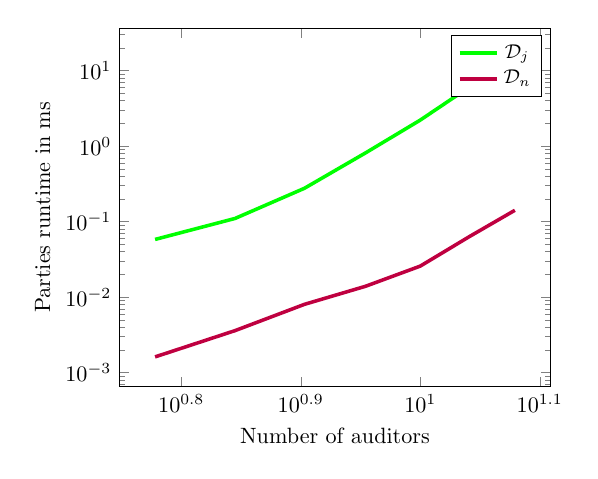
\begin{tikzpicture}[scale=.8]

\begin{loglogaxis}[
	xlabel={ Number of auditors },
	ylabel={ Parties runtime  in ms}
]


%\addplot[green,ultra thick] coordinates {
%  
%%     (1, 0.014)
%     (6, 0.033)
%     (7, 0.033)
%      (8, 0.033)
%      (9, 0.033)
%      (10, 0.033)
%      (11, 0.033)
%      (12, 0.033)
%
%};

\addplot[green, ultra thick] coordinates{

%        (1, 0.019)
       (6, 0.058)
       (7, 0.110)
      (8, 0.276)
      (9, 0.813)
      (10, 2.21)
      (11, 6.1)
      (12, 14.7)
};

\addplot[purple, ultra thick]  coordinates{

%  (1, 0.001)
        (6, 0.001611)
        (7, 0.00359)
      (8, 0.008)
      (9, 0.01389)
      (10, 0.02570)
      (11, 0.0636)
      (12, 0.141)
};


\legend{\small $\mathcal{D}_{\st j}$,\small$\mathcal{D}_{\st n}$,\small $\mathcal{DR}$}
\end{loglogaxis}
\end{tikzpicture}
\end{center}}
\caption{\small Parties' runtime in the PwDR.}\label{plot::runtime}
\end{figure}









